\chapter{Introduction}

\iffalse
Origins have long fascinated the human mind. Something else here.

To fully understand our history, we would hope to understand 1. how we, individually, became conscious; 2. before that, how we developed into human beings; 3. before that, how life began on Earth; 4. before that, how Earth and the Solar system formed; 5. before that, how the Sun formed; and 6. before that, how the Universe formed. The first and final of these questions are generally beyond the scope of traditional Western science, although some neuroscientists and cosmologists (as well as religious scholars, seekers, and philosophers) still try. The second and penultimate questions - how the species (the host of our consciousness) and the Sun (the host of our bodies) came to be - mirror one another both poetically and in that scientists seem to have a fairly solid grasp on each of them, using Darwin's theories and the Hertzprung-Russell Diagram to chart the evolution of our species and our host star. At the center of these six questions, how Life and Earth came into being, we find another symmetry, perhaps most notably thanks to the fact that it is here that science and (Abrahamic) religion disagree most strongly: to the religious mind, the Earth and Life were divinely Created, drawn out from Nothingness into their current, stable forms, while to modern science, life seems to have been the result of some fortuitous chemical mixing and our home, the Earth, the simple by-product of an inefficient stellar formation process somewhere in the suburbia of a minor galaxy in an infinitely vast Universe, both still evolving and changing.



This thesis is an exploration of a miniscule step in the modern Western science's process of finding an acceptable solution to the question of how the Earth and Solar System formed.
\fi

Planetary systems, including our own Solar System, are born from the circumstellar disks of gas and dust that form around young stars. Protoplanetary disks, or proplyds, are young ($\leq$ 10Myr) circumstellar disks, which are characterized by their large abundance of gas, which typically outweighs the disk's dust by a factor of 100. However, as these disks are influenced by gravitational, chemical, and viscous forces, their gas quickly dissipates and the disks become stabler, nearly gas-free debris disks, like our familiar local Solar System. But while we can observe with relative ease the current state of our local debris disk (the Solar System), understanding the process that brought us here - the nature of our proplyd, four and a half billion years ago - is more difficult. To understand this mystery, we must turn to observations of other comparable proplyds, the studies of which can give us insight into the processes and conditions necessary for planet formation.

Indeed, to understand the birth of our proplyd, we must understand the birth of our Sun, as the two are intimately related. Stars form when a region of an enormous molecular cloud develops a gravitational instability sufficient to lead to a runaway collapse (reference). In this process, the cloud shrinks by a factor of around ten million on its way down to a star, analagous to shrinking a square the approximate size of Connecticut ($\sim$150x150 km) down to just 15mm on each side, leading to a tremendous increase in rotational velocity in order to conserve angular momentum. As the local material begins to self-gravitate, its center forms a dense core which will eventually become a young star (binaries are also a common outcome in this process; approximately half of all stars are found in binary systems (Duchene & Kraus 2013)). However, the collapse also leads, almost inevitably (reference), to a circumstellar disk, needed to shed the angular momentum from the protostar to keep rotational velocities from getting too high. These proplyds present flared radial structures, typically extending several hundred AU (vincente & Alves 05 reference). Temperatures in their outer reaches are typically in the 10-100 K range; masses range from ones to tens of Jovian masses (Andrews and Williams 05). Since these disks form directly out of the collapse process, they, like their stellar host and the initial molecular cloud, are composed almost exclusively of molecular hydrogen.

After around ten million years, the gas in these disks tends to deplete almost entirely, through processes including accretion onto the host star, blowing out from radiation pressure, and becoming locked up in rocky bodies, transitioning the disk from a protoplanetary disk to a debris disk. These new debris disks are made up of what is thought to be second generation dust, created by the grinding down of boulders and planetesimals, since any primordial dust from the initial collapse would likely have been blown out by this time. With a few notable exceptions, these disks have no detectable gas. For a more complete review of disk evolution, see Hughes et al (2018).





\section{Submillimeter Observations}

Although proplyds' \textit{relative} dust abundance is low, the actual amount of material that they harbor early in their lives is quite substantial. This makes it difficult to get much information from optical observations of these disks, since at these wavelengths the dust is optically thick. However, since that dust is a bad absorber of millimeter-wavelength emission, observations in the radio band offer us the chance to peer deep into these proplyds as if the dust was not there. In the radio, we may trace two types of emission:

\begin{itemize}
  \item \textsc{Continuum emission}: Although the dust does not absorb at radio frequencies, it is a faint emitter. We call this continuum emission since the signal spans a wide range of frequencies.

  \item \textsc{Line emission}: Thanks to the low temperatures in these proplyds, complex molecules may live a stable existence. We may observe the emission that these molecules emit from rotational transitions, as they de-excite and enter lower energy levels. Conveniently, emission from these de-excitations comes at extremely precise and well-known frequencies, making it easy to identify emission from known molecular transitions in a spectrum. Observations of line emission can provide us with a wealth of important information, including velocity profiles, temperature information, and total disk mass.
\end{itemize}

Notably absent in both forms is emission from the central star, thanks to the fact that stars are extremely weak emitters in the radio regime. Fig \ref{fig:SED} presents a spectral energy distribution, or SED, showing emission intensity as a function of wavelength from an imaginary disk system. As one may easily see, the star's emission is brightest at shorter wavelengths and is almost entirely absent in the 100-1000+ $\mu$m wavelength range, where radio telescopes observe and where disks emit.

\begin{figure}
\centering
  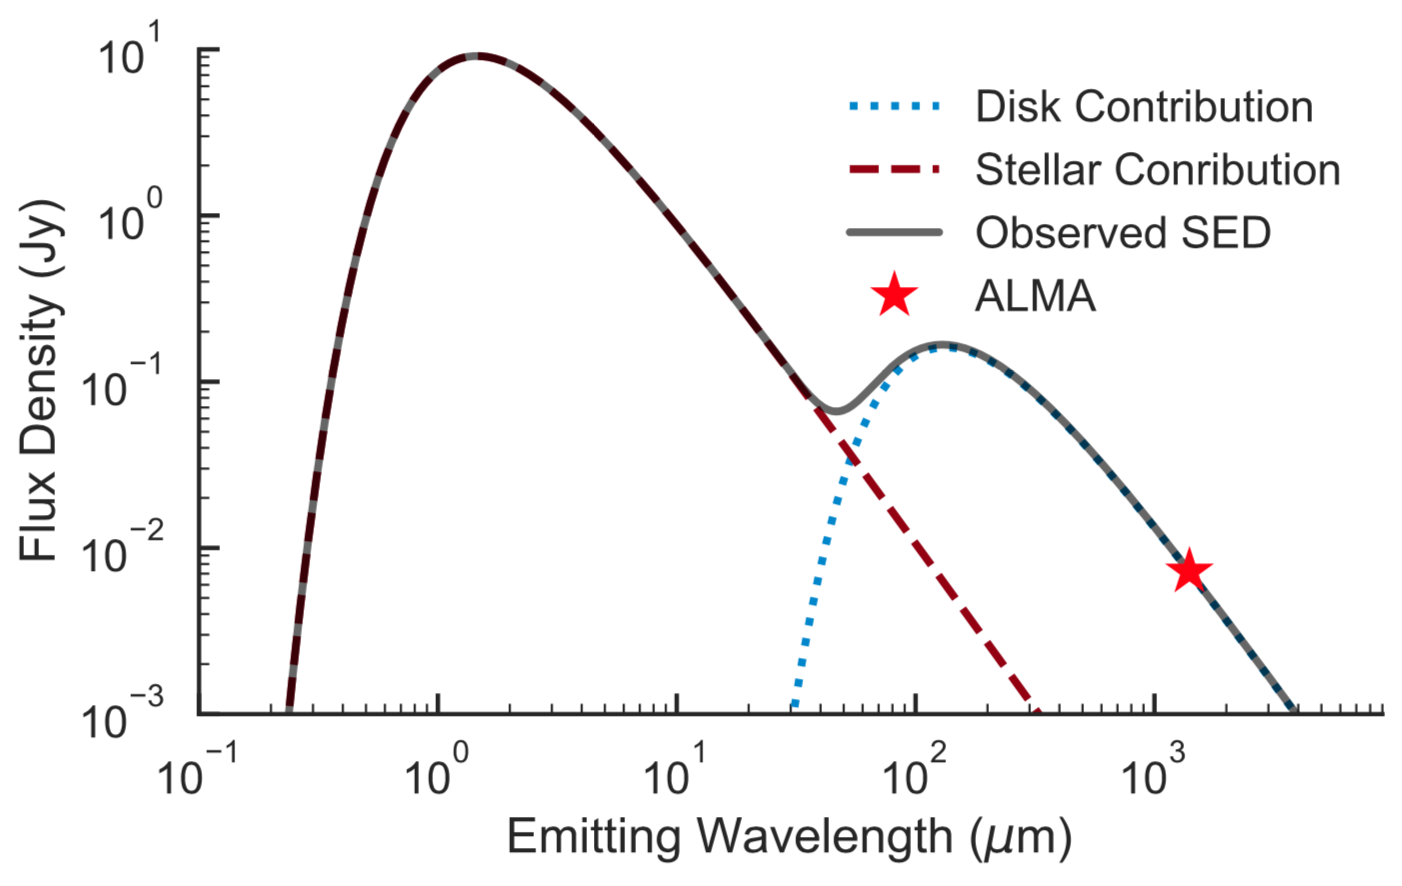
\includegraphics[width=\linewidth]{example_SED.png}
  \captionof{figure}{An example of a spectral energy distribution, or SED.}
  \label{fig:SED}
\end{figure}

However, to understand these types of observation, one must first understand the nature of the $''$telescope" making the observations. What follows is a brief introduction to radio interferometry, followed by a deeper explanation of continuum and line emission.



\subsection{Interferometry}
\label{section: interferometry}
Interferometry is a clever way to make extremely high-resolution observations at long wavelengths without needing to use incredibly large collecting areas. Were one to naively attempt to create a conventional telescope to capture radio emission, they would quickly recall that, for a telescope with a single circular aperture, maximum angular resolution is given by

\begin{align}
  \theta &= 1.22 \, \frac{\lambda}{D},
\end{align}

\noindent where $\theta$ is the angular resolution achieved, $\lambda$ is the wavelength of the emission being observed, $D$ is the diameter of the aperture. Unfortunately, light in the radio regime has wavelengths on the order of millimeters to centimeters, orders of magnitude longer than the hundreds of nanometers that that is typical of emission from optical sources. Consequently, to achieve a resolution comparable to that of an optical telescope, one would have to increase their aperture's diameter accordingly to match the increase in $\lambda$. Some have tried this approach: the Arecibo Observatory in Puerto Rico and the Five hundred meter Aperture Spherical Telescope in China (with diameters of 300m and 500m, respectively) are two immediate examples, but both still have extremely coarse resolution: \~25$''$ for Arecibo and \~15$''$ for FAST, observing 3cm emission. Building and maintaining apertures this big is also an extreme challenge, requiring mountains to be hollowed out, making this an unappealing solution.

The alternative, of course, is to leverage the power of interferometry for a solution to the problem. In an interferometric system, one may reconstruct an image using the interference patterns between light received by two or more separate apertures. In this case, the maximum angular resolution becomes proportional to the maximum distance, or baseline, between any two  apertures, which can be made almost arbitrarily large.

While this interference process can be done at optical wavelengths with CCDs, it is far more difficult to execute, as light must be forced to physically interact before reaching the sensor via a complex, and extremely precise, optical system. At longer wavelengths, however, heterodyne receivers may be used, making task of interfering the signals a digital process, rather than a physical one. A heterodyne receiever records both the amplitude (analogous to the intensity that a CCD might measure) and the phase of the signal it receives. Because the receiver now captures phase information as well as amplitude, the two signals may be digitally interfered after being received. Physical features must be callibrated out, including phase delay caused differences in line-of-sight path length from the source between the receivers, atmospheric effects, and instrumental phase delays.


The output from this process - the complex voltage describing amplitude and phase of the interference pattern caused by interfering light from two telescopes - is called a visibility and lives in the visibility domain, much in the same way as a pixel is the basic unit of the image domain. While the image domain - that familiar world of pictures made up of little chunks of light - has spatial dimensions (i.e. the $xy$ plane), the visibility domain is a bit different, drawing on the $uv$ plane instead. The $uv$ plane is a wavelength-scaled $x-y$ coordinate system parallel to the sky in the direction of the target source. Here $''$wavelength-scaled" can be taken to mean that $u = X/\lambda, v = Y/\lambda$, where $\lambda$ is the wavelength of observation and $X$ and $Y$ are the lengths of the x/y components of the projected baseline. Thus, each baseline samples a specific spatial frequency, given by its position in the $uv$ plane. An interferometer may thus be represented on the $uv$ plane as a scatter of points, which each point corresponding to the wavelength-scaled, target-projected, component distance between two receivers. The ideal receiver would completely fill the $uv$ plane, so that every spatial frequency was sampled. However, since the number of baselines we may access is very limited (approximately the square of the number of antennae in an array), this is clearly an impossibility.

However, the fact that the $projected$ baseline is really what determines visibility's location in the $uv$ plane, rather than the baseline's $''$true", un-projected length, allows us to cleverly gain far more points in the $uv$ plane than one might immediately expect. Since the Earth rotates throughout the night, the projection of a given baseline relative to the target source will change throughout the night as well. Consequently, by making observations over the course of a night, many more points in the $uv$ plane may be sampled, thus giving a better-filled plane. This process is known as $''$Earth rotation aperture synthesis."

We would now like to consider to to recover an image from a set of observed visibilities. In general, moving between frequency space and distance space is given by a simple Fourier transform. When considering this translation for telescopes, we consider the shape of the image produced by observation of a single point source. For a conventional telescope with a circular aperture, coverage in the $uv$ plane is in the shape of a filled circle of constant amplitude. Translation to the image domain, via a Fourier transfer of that shape, results in the familiar 2-D Airy Disk. With an interferometer, this process would be equally straightforward if the $uv$ plane were fully sampled, but because it is not, the resulting image is instead a Fourier transform of all the points in the $uv$ plane sampled by the baselines, and can take on a very complex shape\footnote{Additionally, thanks to the incomplete samplimng of the $uv$ plane, an infinite number of images could all be consistent with some given finite set of visibilities, although many of them would not be physically possible. The one we choose to look at is determined by our deconvolution process, but is not actually the true image.}. As we increase the number of $uv$ points sampled, the resulting image, or dirty beam, will begin to look like a bumpy and/or elongated Airy disk.

In a real observing scenario, the Fourier transform of a set of observed visibilities is a convolution of the dirty beam with the true sky brightness pattern (which is what we really want to find). The process of removing the influence of the dirty beam, and the artifacts it can introduce, is called deconvolution. In practice, this deconvolution process takes the form of some iterative algorithm that selectively removes the effects of the dirty beam. The interested reader is directed to the CLEAN algorithm (Hogbom (1974) reference), the first and most popular process (and the one used in this work), as well as the maximum-entropy method (e.g. Wernecke & D’Addario (1977 reference), Skilling & Bryan 1984 reference).

In summary, interferometry works by recording amplitude and phase information about some emission with many radio antennae and digitally interfering each antenna's signal with the signal received by every other telescope. Each of the resulting interference patterns is called a visibility, and represents a point in $uv$ space. Translation from the visibility domain to the image domain involves combining the Fourier transform of each point and deconvolving the dirty beam's influence. Finally, one is left with a clean science image.

Currently, the world's most advanced interferometer, and the source of this thesis' data, is the Atacama Large Millimeter/Submillimeter Array (ALMA), seen in Fig \ref{fig:ALMA}. Built in the high Chilean desert at around 5,000 meters (16,000 feet), the \$1.4-billion dollar array first opened its eyes for scientific observation in mid-2011, with funding from a global partnership between Chile, the United States, Europe, and several other countries. With its 66 total antennae (50 12-m dishes and 16 at 7-m) and baselines extending out to 15-km, it offers an order of magnitude increase in sensitivity and resolution over previous arrays, which include the Jansky Very Large Array (27 25-meter dishes), the Submillimeter Array (8 6-meter dishes), and the CARMA (23 dishes of 3.5-m, 6.1-m, and 10.4-m diameters).

\begin{figure}[htp]
  \hspace*{\fill}%
  \subcaptionbox{\label{fig:ALMA}}{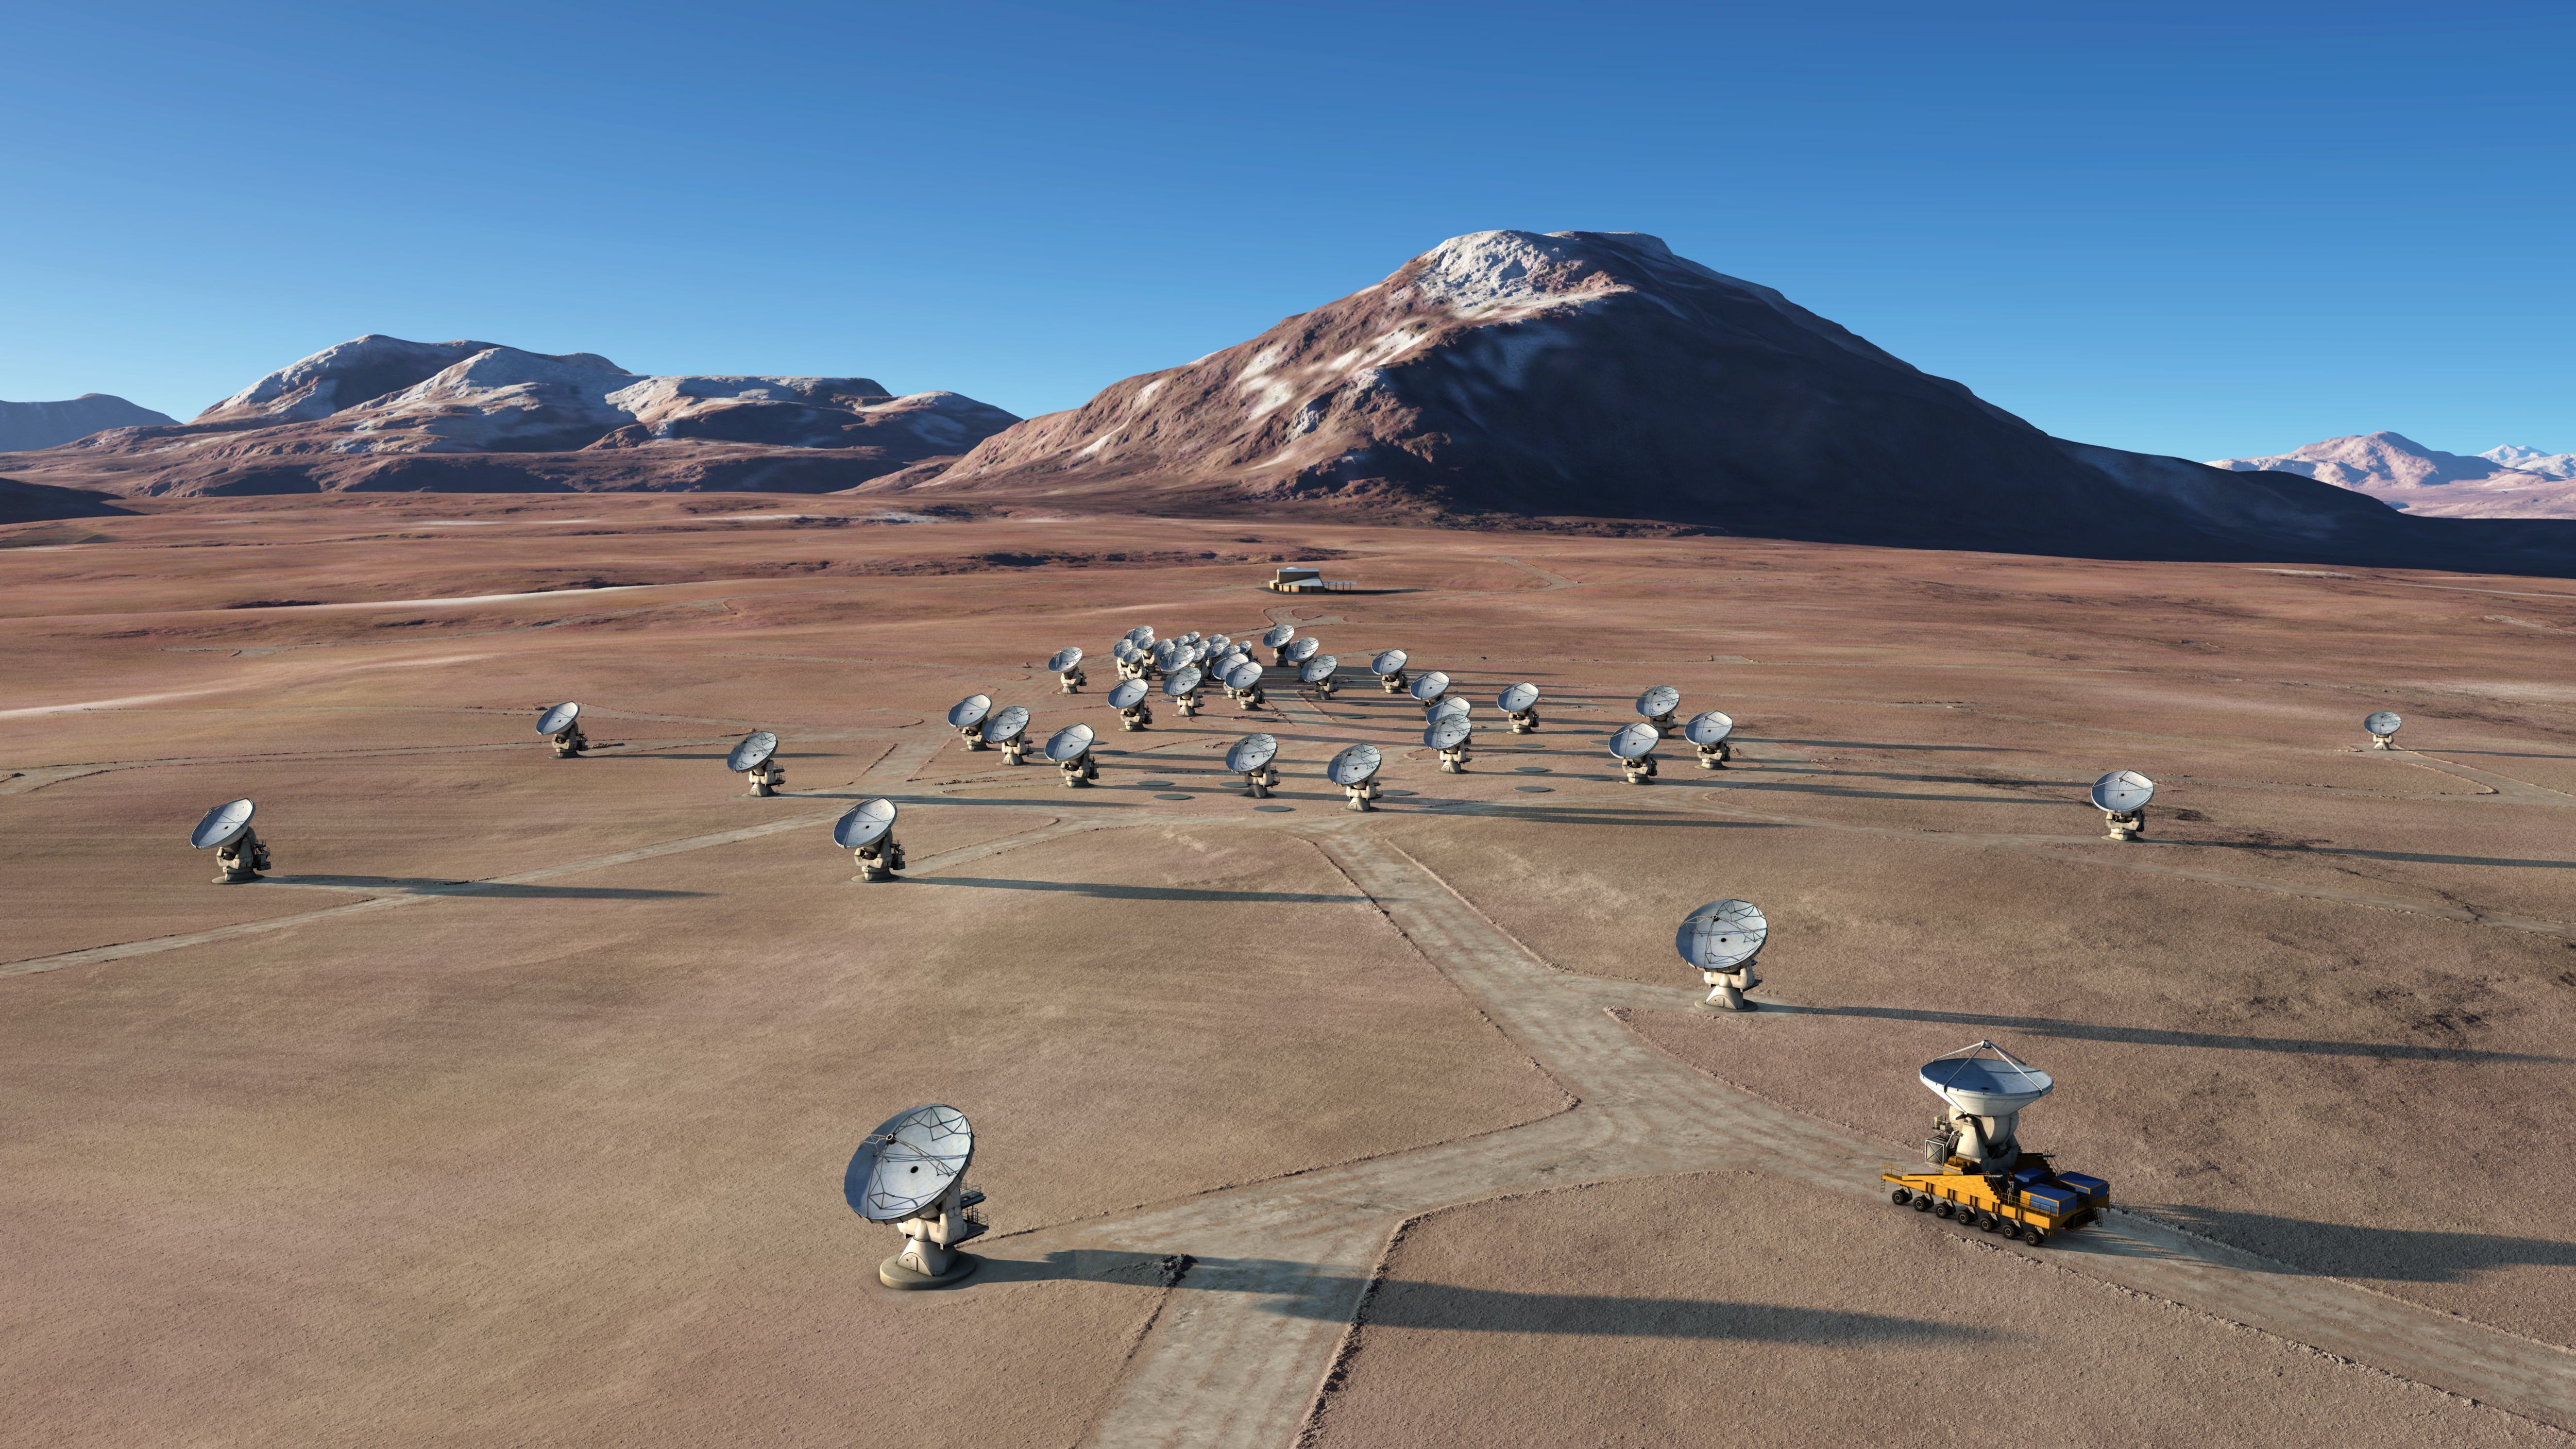
\includegraphics[width=0.5\linewidth]{ALMA_universetoday.jpg}}\hfill%
  \subcaptionbox{\label{fig:Andrews_proplyds}}{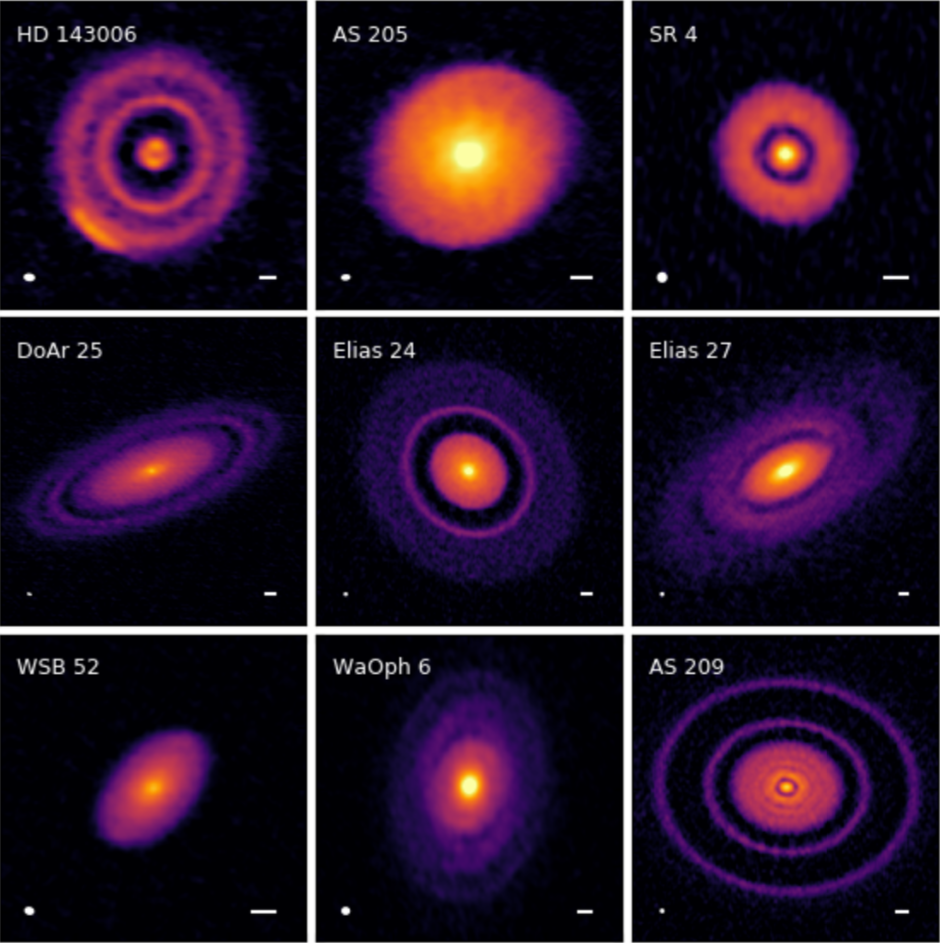
\includegraphics[width=0.3\linewidth]{Andrews2018_proplyds.png}}%
  \hspace*{\fill}%
  \captionof{figure}{Left: A rendering of ALMA shows the interferometer's antennae in the high desert, as well as a purpose-built truck moving one of the antennae (lower right). Right: A recent survey from ALMA reveals stunning detail in several protoplanetary disks.}
\end{figure}


The effects of this increase are striking; gaps and rings in faraway disks are now resolvable in striking clarity (ALMA Partnership et al 2015 reference; Fig. \ref{fig:Andrews_proplyds}), Einstein rings observed in incredibly high-resolution (e.g. Tamura et al 2015, Dye et al 2015, many others reference), and the search for and detection of complex organic molecules in distant proplyds (Oberg et al 2015 reference) is no longer science fiction. These awe-inspiring projects are a small portion of ALMAs contributions to the world of radio astronomy, and more are being made with each passing day.


% \begin{figure}
% \centering
% \begin{minipage}{.48\textwidth}
%   \centering
%   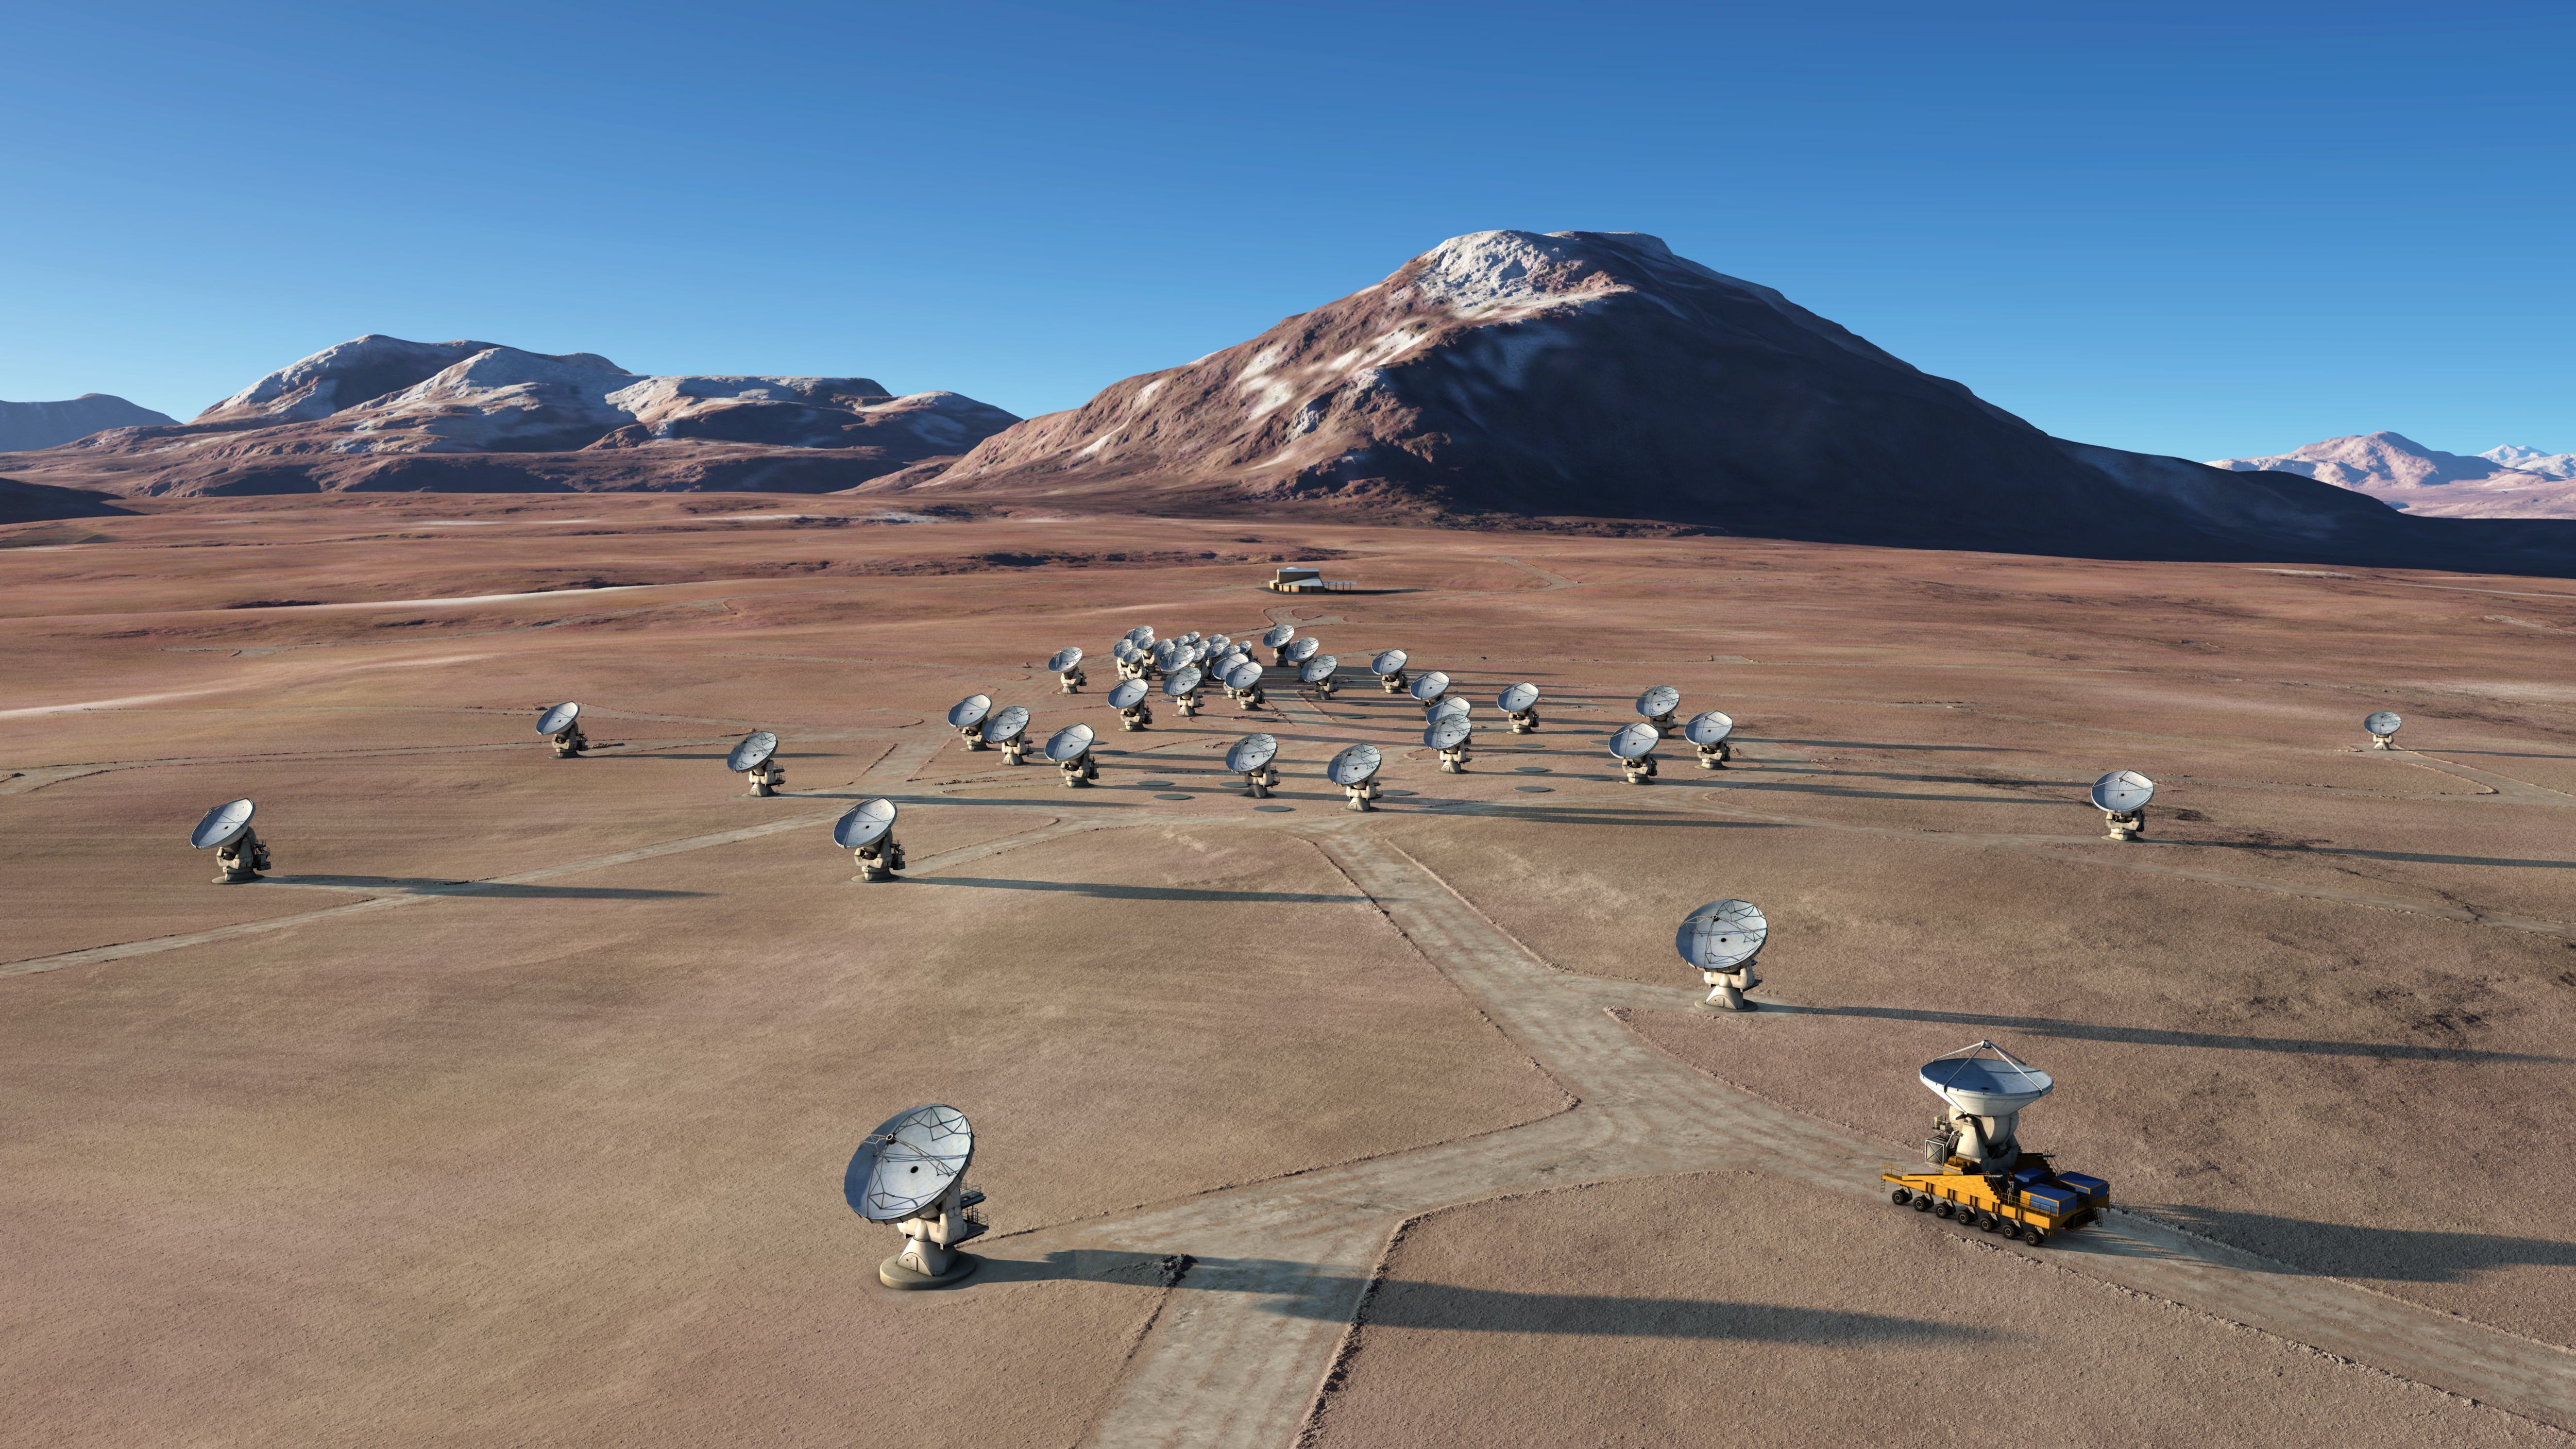
\includegraphics[width=\linewidth]{ALMA_universetoday.jpg}
%   \captionof{figure}{A rendering of ALMA. Antennae may be moved using a large truck, as seen in the lower right corner.}
%   \label{fig:test1}
% \end{minipage}%
% \begin{minipage}{.27\textwidth}
%   \centering
%   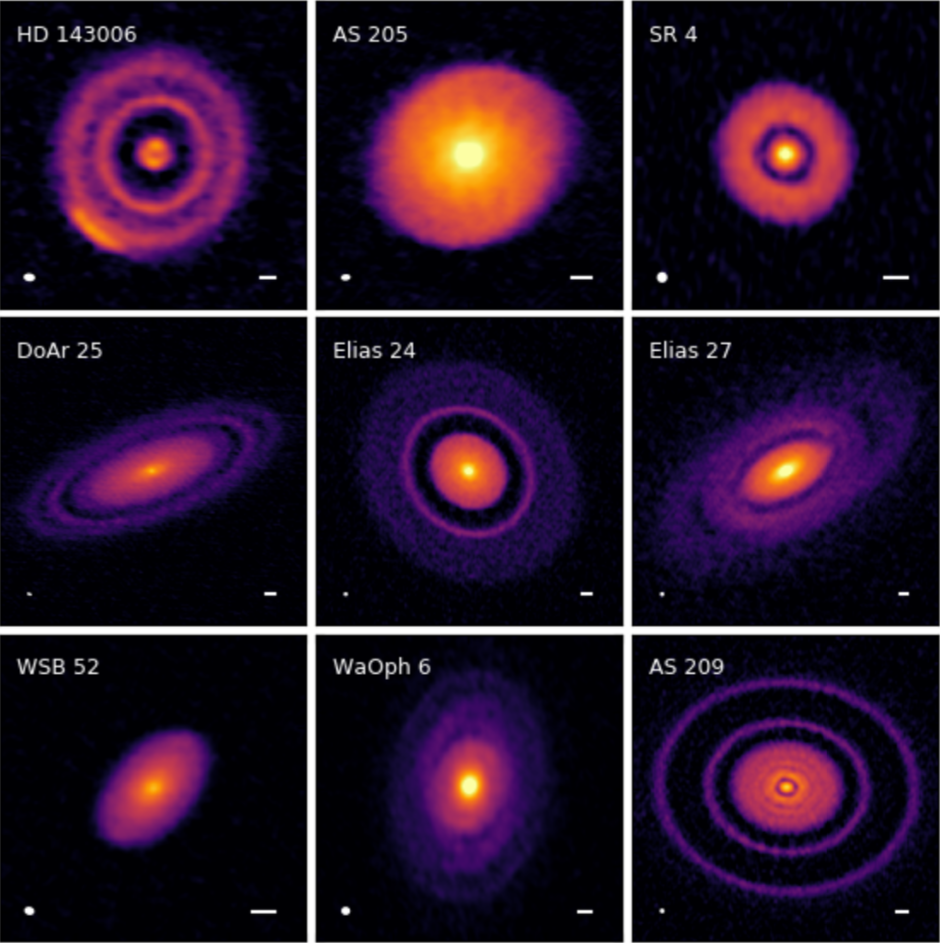
\includegraphics[width=\linewidth]{Andrews2018_proplyds.png}
%   \captionof{figure}{Impressive images of disks from Andres et al (2018)}
%   \label{fig:test2}
% \end{minipage}
% \end{figure}




\subsection{Continuum Emission}

Continuum-emission observations integrate flux from a wide band of frequencies, much like an image in the optical would. They are appealing for their simplicity and because they are sensitive to faint objects.

When observing proplyds, an understanding of planet formation is often a guiding motivation. One parameter that is critical to the planet-forming process is total disk mass. We know that, to first order, when a disk is optically thin, its total mass, $M_{\text{disk}}$, is linearly proportional to its flux density, $F_{\nu}$ (reference Hildebrand 1983), found from an observation of continuum emission. This relationship is given by

\begin{align}
M_{\text{disk}} = \frac{F_{\nu} d^2}{\kappa_{\nu}\ B_{\nu}(T_c)},
\end{align}

%below: really opacity power law index, but simpler this way and they mean the same thing.
where $d$ is the source's distance, $\kappa_{\nu}$ is an assumed dust opacity, and $B_{\nu}(T_c)$ is the Planck function at a given charatcteristic temperature, $T_c$. The value of $T_c$ and disk opacity can be inferred without much difficulty by fitting the proplyd's SED using a simple model. This function is, of course, rather approximate; it assumes a single temperature and single dust opacity (a function of composition and grain size distributions) throughout the disk. The assumption of optically thin emission means that calculations made will inherently be lower limits, since any substantial optical depth will block emission from inner regions of the disk. Futhermore, even in the case of optically thin emission, significant mass may be locked up in bodies that are invisible to our observations. Still, it is a useful tool that can be used to approximate disk mass using continuum-emission images.


\subsection{Line Emission}

As molecules interact with one another or absorb light, they gain energy, entering higher rotational energy states. However, as their presence in these states cannot be sustained without the addition of more energy, they will de-excite soon after. This de-excitation process - stepping down from one rotational energy state to the one below - causes the emission of light. Every transition in every molecule emits at its own specific frequency, or rest frequency, making that light identifiable to observers. We may observe a specific rotational transition from a single type of molecule by tuning our receiver to be sensitive to a very narrow window of frequencies immediately around the rest frequency of the transition of interest. While this limits the amount of flux we may receieve, the information gained about that origin of that signal is valuable.

One immediate feature that line emission gives us access to is velocity information: since all emission should have a single frequency (the transition's rest frequency), we immediately know that any variation from that central frequency is a result of Doppler shifting caused by line-of-sight velocity. This allows us to make a $''$moment-one" map of emisison, tracing velocity in the disk (Fig \ref{fig:m1map})

%\begin{wrapfigure}
\begin{figure}[htp]
  \hspace*{\fill}%
  \subcaptionbox{\label{fig:m1map_hco}}{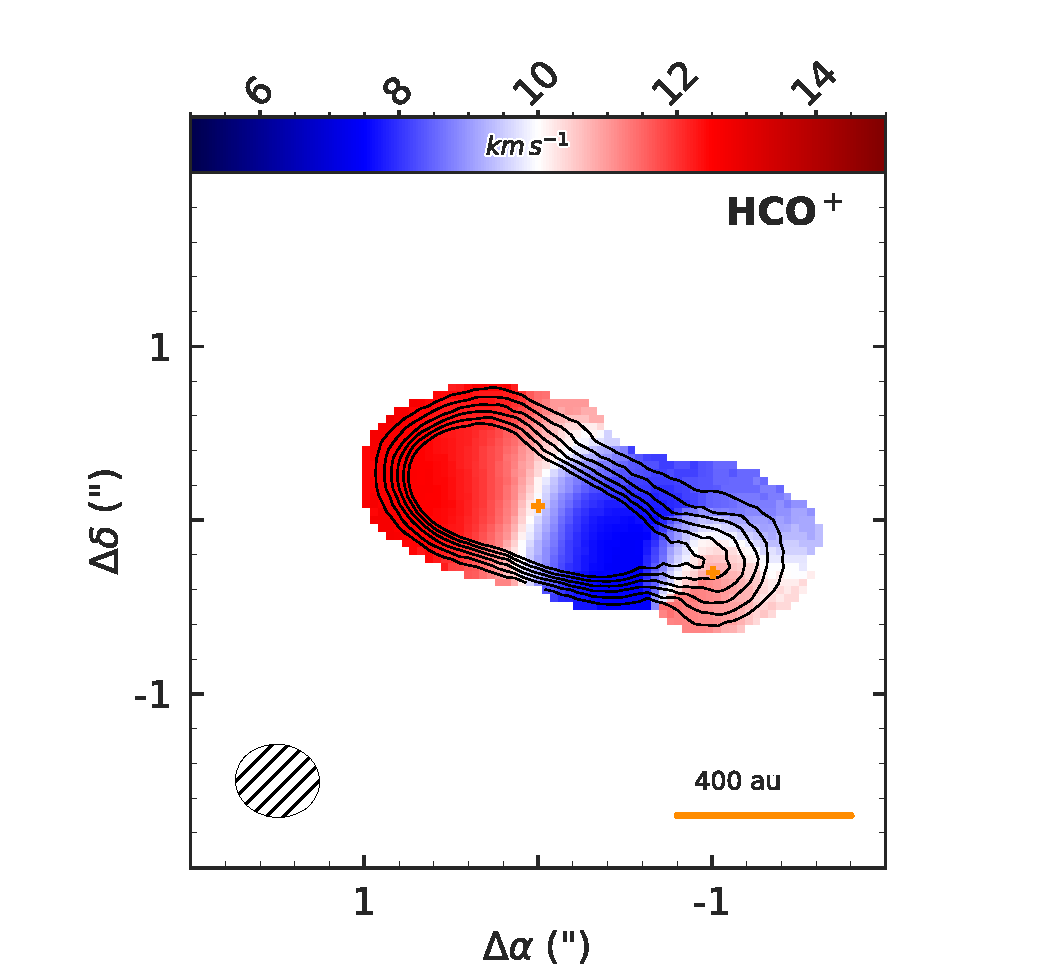
\includegraphics[width=0.25\linewidth]{m1-map_hco.pdf}}\hfill%
  \subcaptionbox{\label{fig:m1map_hcn}}{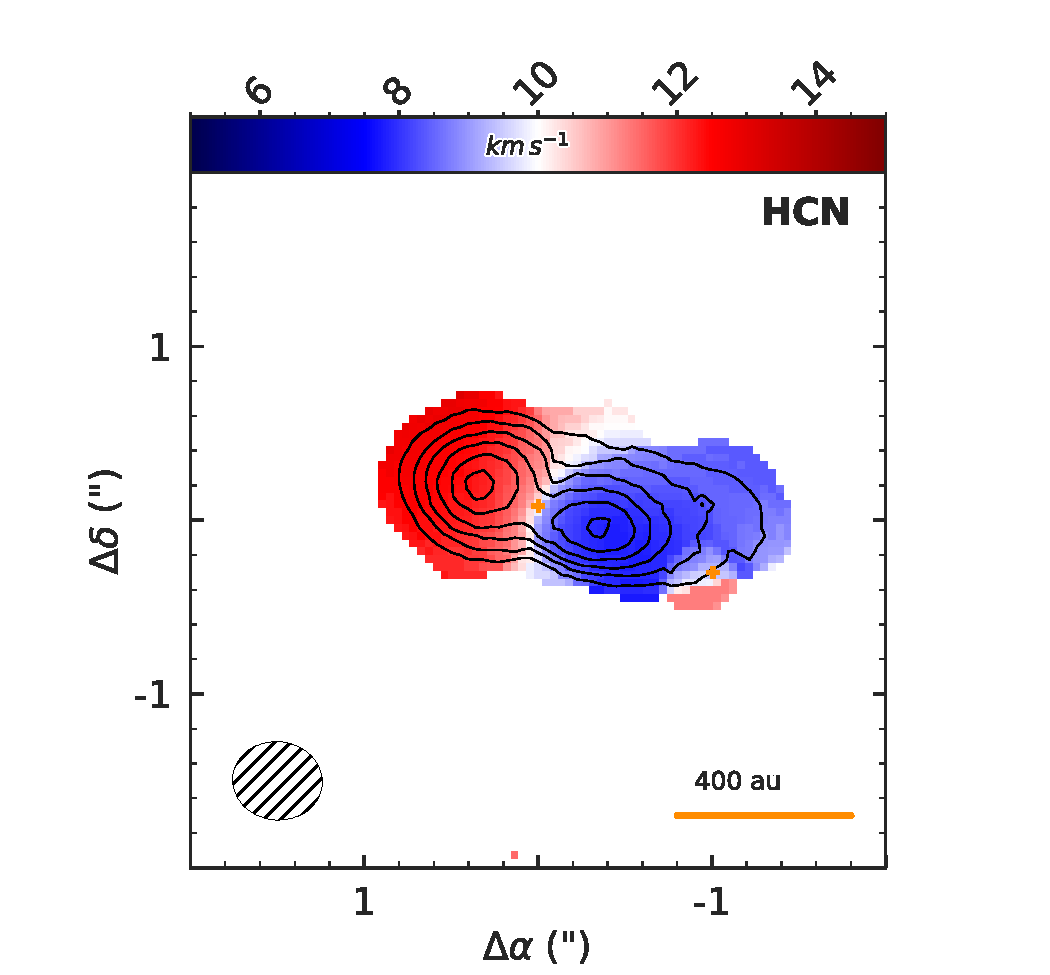
\includegraphics[width=0.25\linewidth]{m1-map_hcn.pdf}}\hfill%
  \subcaptionbox{\label{fig:m1map_co}}{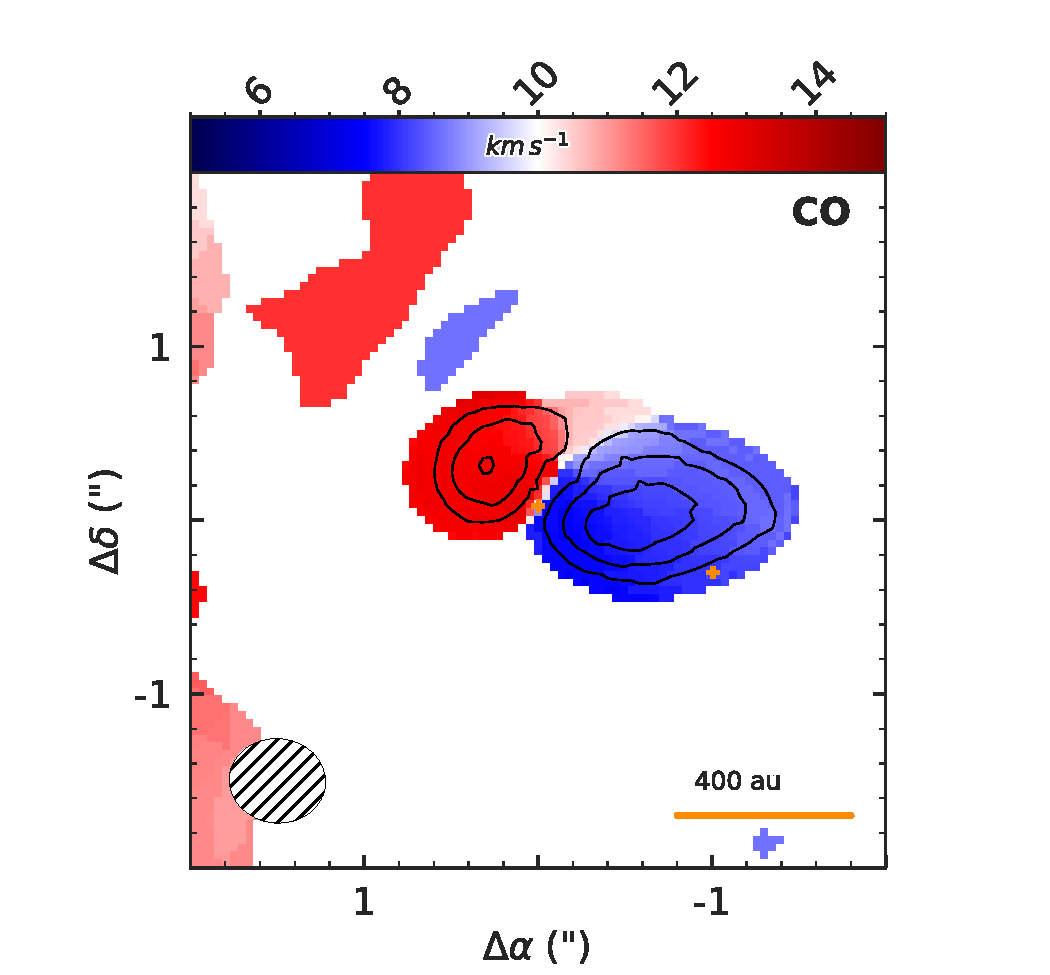
\includegraphics[width=0.25\linewidth]{m1-map_co.pdf}}\hfill%
  \subcaptionbox{\label{fig:m1map_cs}}{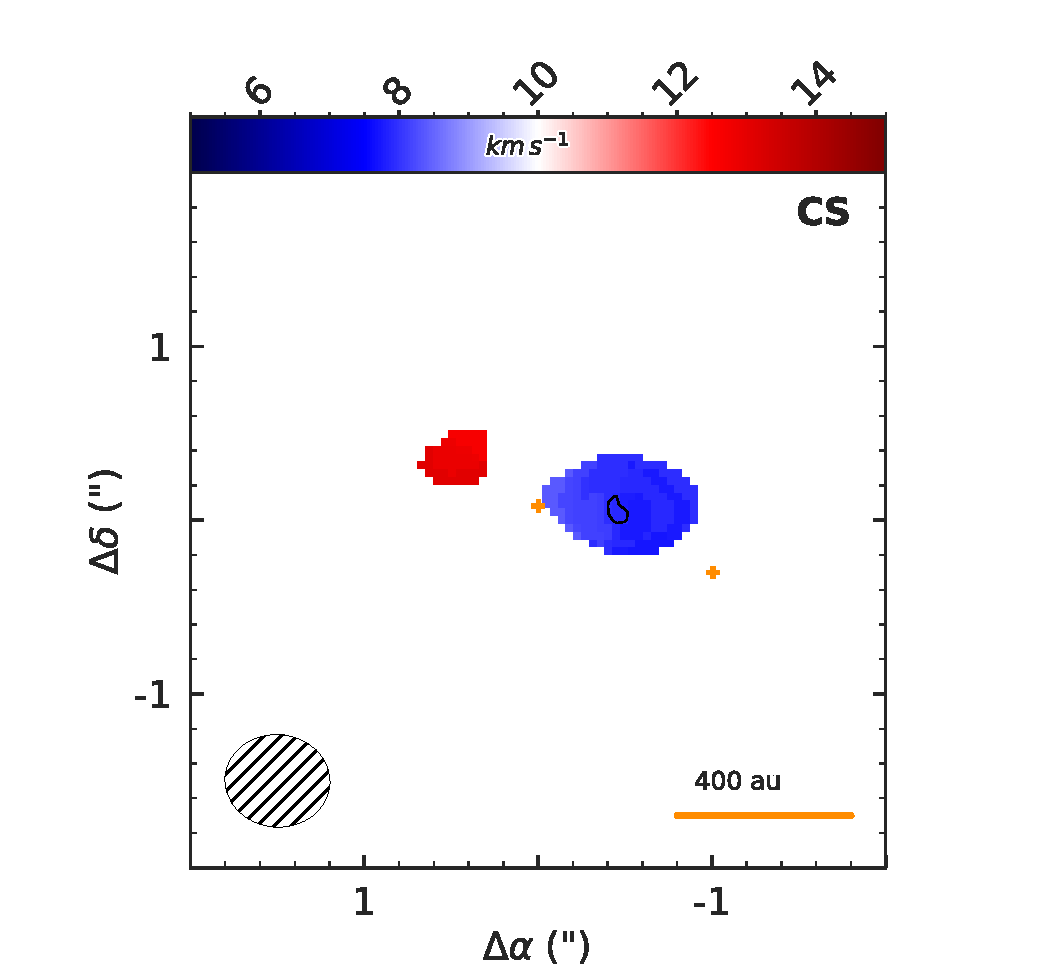
\includegraphics[width=0.25\linewidth]{m1-map_cs.pdf}}\hfill%
  \hspace*{\fill}%
  \captionof{figure}{Moment-1 maps of HCO$^+$, HCN, CO, and CS emission (left to right) in the present study's proplyds.}
\end{figure}
%\end{wrapfig}

Observations of line emission also give us information about both the temperature and density structures of the disk, since these are the two factors that influence how much emission we may observe. However, in optically thin emission, the two are degenerate, since an increase in either one will increase emission intensity. In this case, we may combine observations of multiple species to model the temperature. In the case of an optically thick line, however, the temperature and density are no longer degenerate, since all emission originates from the $\tau=1$ surface, which removes density from the equation and gives us a value for the temperature at that point in the disk's vertical structure.

Besides offering information about density and temperature, line emission also provides another way of finding disk mass. Like the initial cloud that the star and proplyd formed from, the vast majority of the disk's mass comes in its gas, and like that initial cloud, the vast majority of that gas is molecular hydrogen, or H$_2$. However, since H$_2$ is a symmetric molecule and thus has no permanent dipole moment, it has no rotational transitions and does not emit in the radio, making it invisible to our instruments. As a consequence, we must instead observe emission from other molecules, make assumptions about relative abundances of that molecule to H$_2$, and extrapolate the total disk mass from there.

The second most abundant molecule behind H$_2$ is CO. Thanks to its abundance, as well as its relatively low excitation temperature, CO provides robust, bright emission. Drawing on measurements of CO/H$_2$ ratios in warm dense cloud (e.g. Aikawa & Herbst 1999; Fogel et al. 2011 reference), we use a ratio of 1:10000, or 10$^{-4}$, to determine COs relative abundance in proplyds. Ratios for less prominent molecules with more complicated chemistry (including HCO$^+$, HCN, CS, CN, methanol, and others) are drawn from the interstellar-medium literature and chemical modeling. It is not certain that these values are constant either with location or age, but are generally assumed to be.




\section{Disks \& The Role of Environment}

Line observations of proplyds in high-mass star-forming regions (SFRs) provide an incredible opportunity for two significant reasons. First, they are new; not until ALMA opened its 66 eyes were we able to have such a direct and high-resolution view of proplyds in this environment. Second, since there is significant evidence that our own Sun formed out of an high-mass SFR, these constraints will provide useful insights into our own system's evolutionary history. Thus, for both reasons, we would like to better understand the role that environment plays in the development and evolution of proplyds, comparing them to the well-studied disk population in low-mass and the one well-characterized proplyd in a high-mass SFR, and evaluate how that environment may affect planet-formation potential.



\subsection{The Minimum Mass Solar Nebula}

The minimum-mass solar nebula (MMSN) is a rough conceptual aid used to inform astronomers about the distribution of material is required to form a planetary system (MMSN, Weidenschilling 1977). The MMSN is the radial mass profile that our own Solar System would present if the mass of each planet were, rather than being bound up in spheres, instead ground up and spread across the ring bound by the orbits of their inferior and superior neighbors. The resulting mass profile represents the minimum surface density required to form our own proplyd and thus a way to inform our comparisons of other disks to our own. When this surface density profile is integrated into a single mass, it gives $M_\text{MMSN} = 0.01 M_{\odot}$.

It is, of course, an extremely approximate characterization. One significant assumption it makes is that our planets formed in their current positions. This is a statement that we know both to be false (Walsh et al. 2011; Tsiganis et al. 2005) and consequential, since planetary migration can cause disks to lose mass by pushing competing planetesimals either out of orbit or into inner regions of the disk where they may be more susceptible to accreting onto the host star. Still, in spite of this, the MMSN offers us a diagnostic tool in a field that has few, and is generally considered a useful way to determine if a disk has $''$planet-formation potential."


\subsection{Low- and High-Mass Star Forming Regions}
Thanks to limitations in sensitivity and resolution, most submillimeter surveys in the pre-ALMA epoch focused on proplyds in the nearby low-mass SFRs of Taurus-Auriga and $\rho$ Ophiuchus. Dust-emission studies of disks in this regions by Andrews \& Williams (2005, 2007 reference) have yielded a wide range of disk masses, with a median of 0.005 M$_{\odot}$ and a significant fraction with mass greater than the MMSN. This large fraction of disks with planet-forming potential is consistent with what we would expect based on the enormous - and still growing - volume of exoplanets that have been discovered in the last two decades.

Of course, studying only nearby disks paints an incomplete picture of the population and its evolutionary trends; for one, most stars form in high-mass SFRs (Lada \& Lada 2003 reference), and low-mass SFRs are qualitatively different than their high-mass siblings. High-mass SFRs are massive, dense clusters with large abundances of high-mass O and B stars. Proplyds in these regions experience accelerated mass loss, thanks to the powerful ionizing radiation from the high-mass stars and the increased chance of gravitational interaction caused by their high densities (reference maybe?). This mass loss is likely a problem for planet formation (Johnstone et al. 1998 reference), but its effects are not yet well understood. It is because of these factors that we would like to study disks in high-mass SFRs.


\begin{figure}[t!]
\centering
  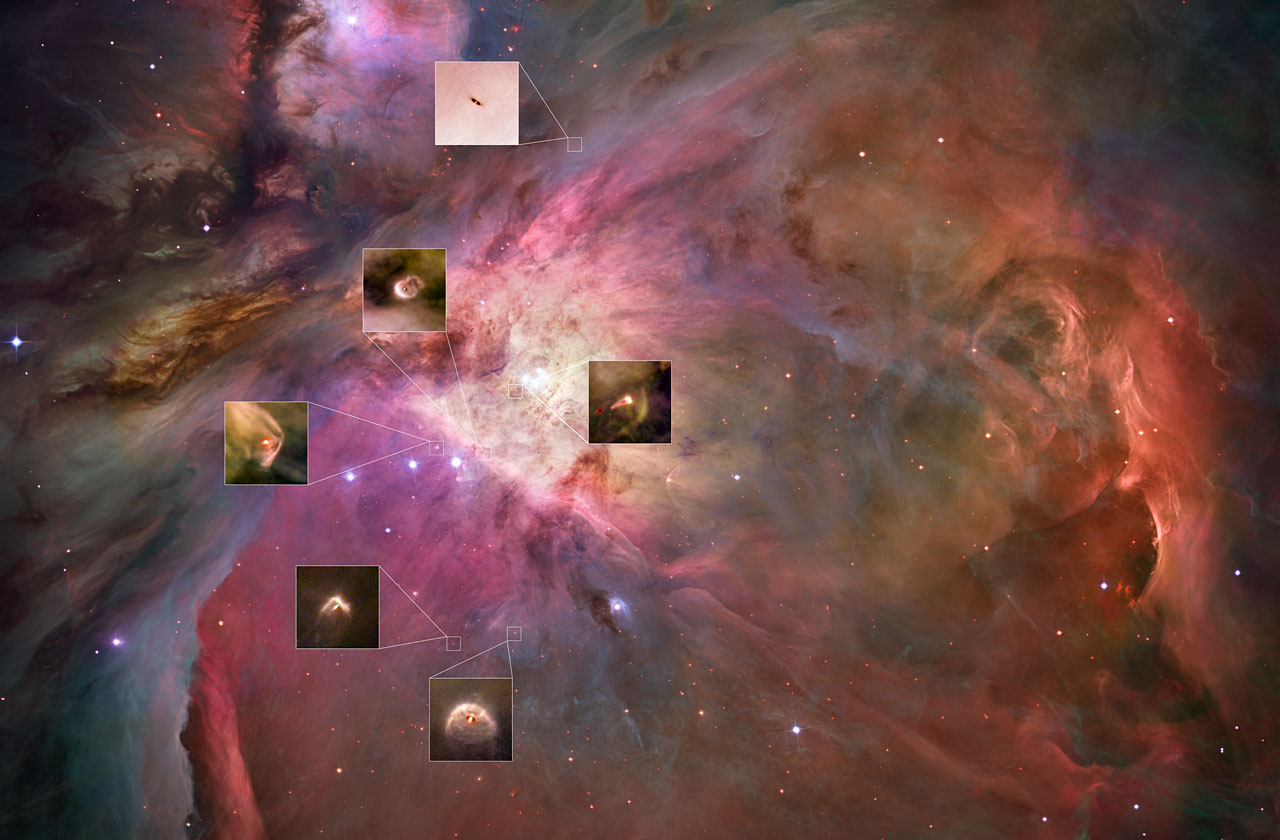
\includegraphics[width=\linewidth]{HST_Orion_proplyds.jpg}
  \captionof{figure}{NASA press image of a selection of proplyds in the Orion Nebula. The closer a proplyd is to a large, bright star, the more visibly "windswept" it is. Image courtesy of HST}
  \label{fig:HST_ONC}
\end{figure}

The nearest high-mass SFR to us is the Orion Nebula Cluster (ONC), 389 pc away. In addition to studies of it in the radio, the Hubble Space Telescope has dedicated significant time to it, producing an abundance of iconic and awe-inspiring images it and of the proplyds it hosts. Many of these proplyds are visibly teardrop-shaped, tailing away from the cluster's biggest, brightest stars. Images like Fig \ref{fig:HST_ONC}, showing disks being pushed away from nearby bright stars, and countless others demonstrate the harsh environment that these young disks exist in, thanks to their local O and B stars.

Indeed, the influence of these large stars has already been demonstrated, both in their affect on mass-loss rate and mass distribution. Statistically-significant anti-correlations between disk mass and proximity to the ONC's central O star, $\theta^1$ Ori C, have been shown using both data from the SMA (Mann & Williams 2009 reference) and ALMA (Eisner et al 2018 reference). Furthermore, observations characterizing mass-loss rates for proplyds in the Orion Nebula have found rates of $\dot{M} \approx 10^{-7}$ M$_{\odot}$ yr$^{-1}$ (Henney \& O'Dell (1999) reference), which implies that a typical disk (i.e. one of MMSN-scale, or $\sim0.01$ M$_{\odot}$) would be fully dispersed before giant planets could form (Hubickyj et al. 2005 reference) and before they could reach the inferred age of the disk-hosting stars in the ONC of $\approx$ 2 Myr (Reggiani et al. 2011; Da Rio et al. 2009 refernce).

Despite all this, not only do we still see disks, but we still see significant planet-forming potential in the Orion Nebula, potential that is comparable to that of other low-mass SFRs. A full 30\% of disks surveyed in the ONC have disks with masses greater than or equal to the MMSN, falling comfortably between $\rho$ Ophiuchus' 29\% and Taurus' 37\% (Andrews & Williams (2005, 2007) reference). This is, of course, a bit of a naive way of comparing them, since although total disk populations may be comparable, it says nothing about the potential for different chemistries and structures typical of the disks in each different region. Still, it is encouraging that the populations are approximately similar.

However, one survey so far has been made of Orion proplyds in molecular line emission (Mann et al 2014 reference).
It studied 22 disks in four lines: HCO$^+$, HCN, CO, and CS. So far, one of the surveys disks has characterized, in Factor et al (2017 referece), where they found some slightly unexpected disk chemistries and morphological structures. The disks that are the subject of this thesis are drawn from the same survey.



\subsection{Relevance to Our Own History}
Understanding the nature of these systems is fundamental to understanding our own past, as there is significant evidence indicating that, like the majority of other stars, our own solar system formed in a high-mass SFR. In Tachibana et al (2006 reference), the authors show that, using iron isotope ratios, our Solar System received ejecta from a supernova in its early history. They do so using $^{60}$Fe, a relatively short-lived isotope of iron that can only be formed in stars. By evaluating $^{60}$Fe/$^{56}$Fe ratios in ferromagnesian chondrules, they are able to infer an initial $^{60}$Fe/$^{56}$Fe ratio, ($^{60}$Fe/$^{56}$Fe)$_0$. This value is consistent with predictions of of levels one would expect from nucleosynthesis in a supernova, indicating that a supernova influenced our early Solar System. Since supernovae come from the implosion of large stars and are relatively rare, the fact that our own Sun was affected by one indicates that it was born in a region that hosted a significant range of stellar masses, as well as having a high rate of stellar formation. While these features are characteristic of high-mass SFRs, they are extremely improbable in low-mass ones, thus indicating that our Sun must have come from a high-mass SFR.


%Gaidos et al. (2009) use levels of 26Al to support this hypothesis though they attribute the levels they see to winds generated by nearby high-mass stars.



\section{d253-1536: A Misalgined Binary System}

The subject of this thesis is the system d253-1536, a misaligned binary of pre-main sequence stars in the Orion Nebula Cluster. Each star in the system has its own proplyd, henceforth called disk A and disk B (left and right, respectively, in all images of the system).

\subsection{Local Environment \& Features}
d253-1536 is located in M43, a nebula adjacent to M42, the famous Orion Nebula and part of the Orion Nebula Cluster (ONC). Many previous surveys have studied disks in the Trapezium cluster, a region near M42's brightest star O-star $\theta^1$ Ori C, and have found a significant truncations of both disk masses, with no disks exceeding $\sim$0.034 M$_\odot$ (Mann \& Williams (2009 reference)), as well as radial extent, with no disks extending out past 60 AU in this region (Eisner et al 2018 reference).

However, because of M43's separation from the Trapezium cluster (it lies $\geq$ 1 pc to the cluster's north), disks in this region do not experience the same levels of photoevaporation. M43 has only one large emitter, Nu Ori, which is a triple-star system whose main component is a B-stype star. d253-1536 is wrapped in an ionization bow shock, HH 668 A, about 1$''$ to the system's west and facing towards Nu Ori, but otherwise the system shows no signs of influence from giant stars, whether in photoevaporation or in morphological influences (Mann \& Williams (2009) reference).

The system's larger disk, disk A (the disk on the left in the images), has a large jet emanating from it in observations in the optical made with HST. However, since the jet is not visibile in the radio, we make no attempt to discuess, explain or model it.



\subsection{Previous Observations}

\begin{figure}[htp]
  \hspace*{\fill}%
  \subcaptionbox{\label{fig:v2434ori_smith05}}{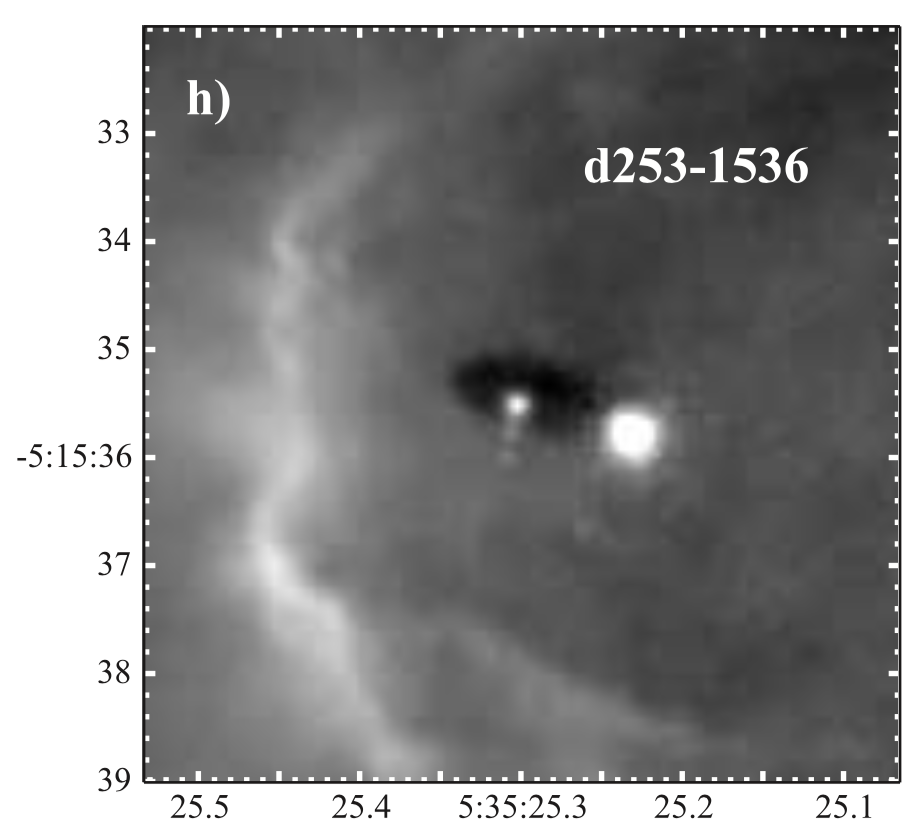
\includegraphics[width=0.33\linewidth]{V2434Ori_Smith05-2.png}}\hfill%
  \subcaptionbox{\label{fig:v2434ori_mann09}}{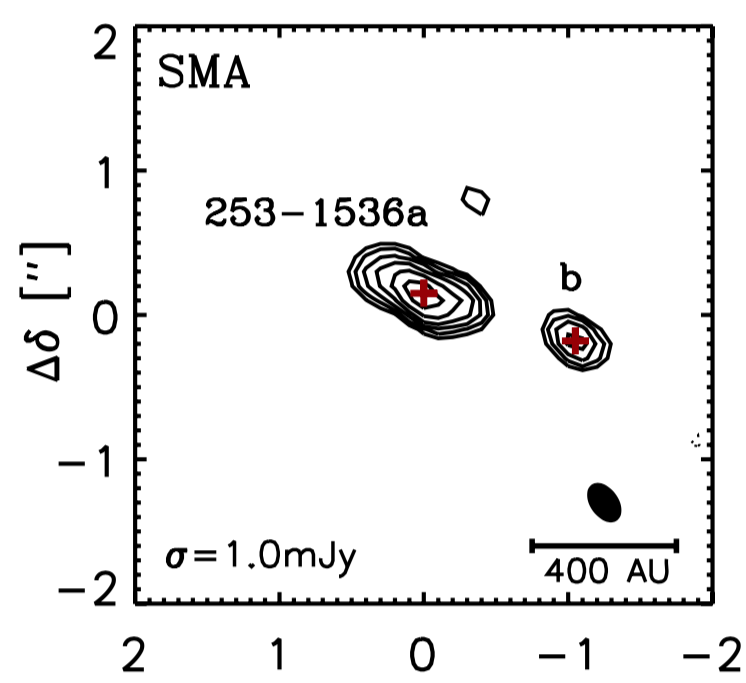
\includegraphics[width=0.33\linewidth]{V2434Ori_Mann09.png}}\hfill%
  \subcaptionbox{\label{fig:v2434ori_ricci11}}{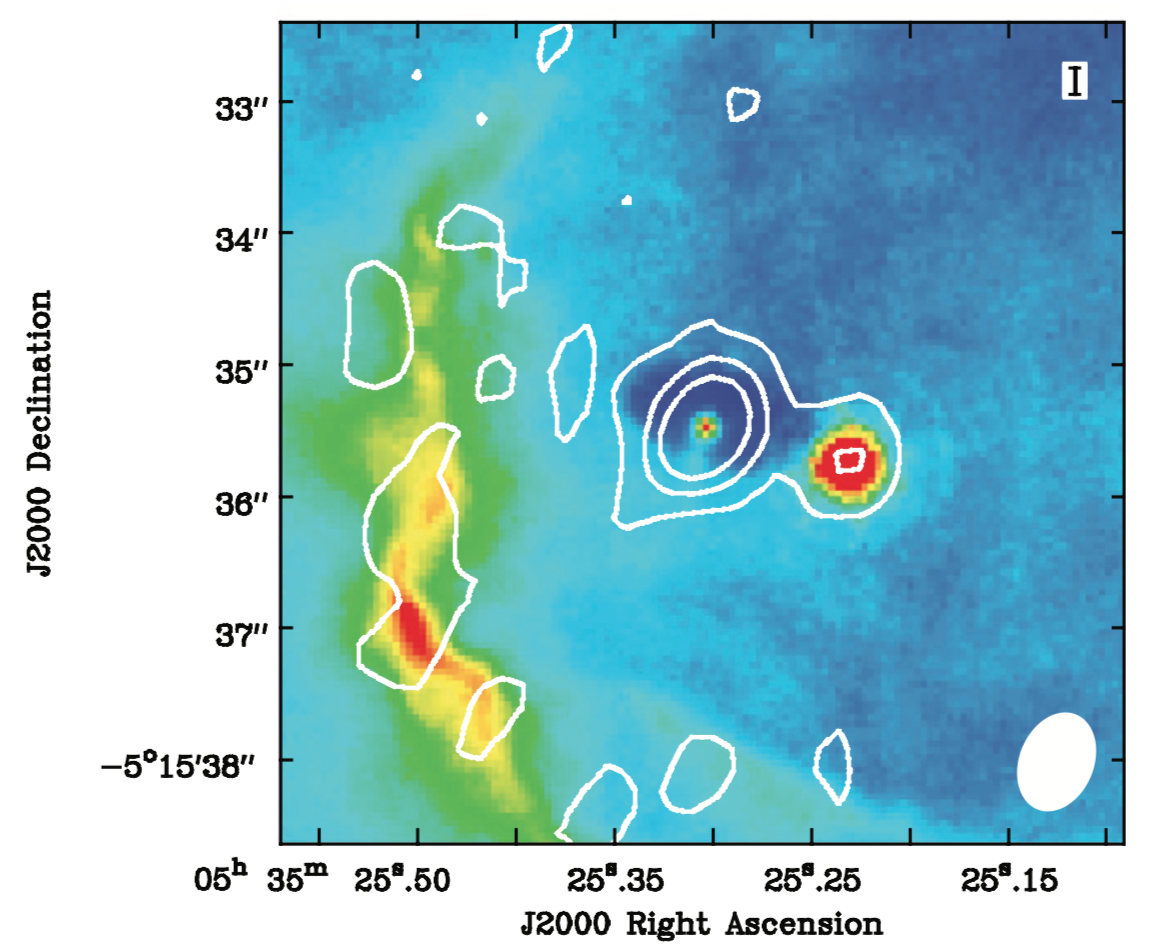
\includegraphics[width=0.33\linewidth]{V2434Ori_Ricci11.png}}\hfill%
  \hspace*{\fill}%
  \captionof{figure}{Images of V2434 Ori taken from Smith et al (2005) on HST (left), Mann et al (2009) with the SMA at 880 $\mu$m (center), and Ricci et al (2011) with the EVLA at 7mm (right). The ionization front is clearly visible in both the HST and EVLA observations, and the jet from disk A is visible in the HST image.}
\end{figure}

First observed by Smith et al (2005 reference) using the Hubble Space Telescope, the authors took interest in what they saw as a binary system containing one star without a disk and one star embedded in a proplyd with a large jet and exhibiting tidal interactions with its companion (Fig \ref{fig:v2434ori_smith05}). Mann \& Williams (2009 reference) used 880 $\mu$m continuum measurements to estimate dust masses of the disks to be 0.066 M$_{\odot}$ and 0.018 M$_{\odot}$, for disks A and B respectively, making d253-1536a the most massive disk measured in the ONC, significantly larger than the Cluster's second largest disk at 0.034 M$_\odot$ and adding credence to the theory that $\theta^1$ Ori C is likely responsible for the truncation of disk masses in the Trapezium cluster. Subsequent detections at 7mm by Ricci et al (2011) indicated that both disks are hosts to substantial populations of large dust grains (\ref{fig:v2434ori_ricci11}), although the distributions of grain sizes are different in the two disks. The same study also spectral typed the host of d253-1536b to be an M2 star and G2 for d253-1536a's host star.

The system was observed in an ALMA survey of 22 proplyds in M43 by Mann et al (2014 reference) in four molecular lines (HCO$^+$, HCN, CO, and CS; Fig \ref{fig:m1map}), and preliminary characterizations were made by Williams et al (2014 reference). Using continuum observations alone and assuming canonical values for temperature, dust opacity, and gas-to-dust ratio, they found disk masses of 0.074 M$_{\odot}$ and 0.028 M$_{\odot}$ for disks A and B, respectively, larger than the previous values. They found an inclination for disk A of $i_A \sim 65^o$, but did not resolve disk B and thus were unable to determine its inclination. They found systemic velocities of 10.55 and 10.85 km/s for the two disks, which are close enough to be well within the escape velocity that the authors calculated for a disks at their projected separation of 440 AU of 2.5 km/s, indicating that the binary is a bound one. This similarity in systemic velocity also indicates that the binary's orbital plane is likely close to face-on.


With our high resolution observations of gas line emission, we aim to determine the temperature, density, and chemical profiles of the system, as well as refining the mass estimates for both disks and host stars. With this information in hand, we will examine this disk's characteristics in the context of previously studied disks in the Taurus and Ophiuchus star forming regions, as well as comparing it to the disk studied by Factor et al (2017 reference), and evaluate the disks' planet forming potentials.






% The disk was discovered by Smith et al. (2005) using HST and is one of the largest and most massive disks in the ONC (Mann & Williams 2009a, 2010; Mann et al. 2014). Smith et al. (2005) determined that the disk is almost edge-on with an inclination of ⇠ 80  75 to the east1 and a position angle of 173 (E of N). They also noted that the northern portion of the disk, as seen in scattered light, is ⇠ 50\% larger than the southern portion. The disk is also associated with HH 667 E, a partial bow shock slightly bent to the south, and HH 667 W, several diffuse filaments along the rotation axis of the disk.

% Continuum observations using the SMA by Mann & Williams (2009a) have marginally resolved the disk and determined its mass to be 0.0450 ± 0.0006 M with a radius of 291 AU. They detected no signs of external photoevaporation, as would be expected from its location far away from any O or B stars. Analysis of continuum data from ALMA (from which gas line data is presented here) by Mann et al. (2014) produced a disk mass of 0.0437 ± 0.0007 M with a radius of 525 AU. Mann & Williams (2009a) also strongly detected the CO(3–2) transition but were unable to separate the disk from the cloud contamination.

% Using observations from the Combined Array for Research in Millimeter Astronomy (CARMA) and the Australia Telescope Compact Array (ATCA), Ricci et al. (2011) were able to fit the long wavelength spectral index to determine a dust opacity index of  = 1.0 ± 0.3, indicative of grain growth. The dust opacity is assumed to be a power law as a function of frequency: ⌫ / ⌫. They also derive a disk mass of 0.02 M.

% With our high resolution observations of gas line emission, we aim to better constrain the mass, as well as determine the temperature and density structure of d216-0939 and the mass of the host star. With this information we will examine this disk, located in the outskirts of the ONC, in the context of previously studied protoplanetary disks located in Taurus and Ophiuchus and compare the planet- forming potential. We also obtain a dynamical mass measurement for this pre- main sequence star which can be compared to theoretical evolutionary tracks.









\section{Summary of Contents}

In this work we characterize ALMA observations of two young protoplanetary disks in the d256-1536 system. Observations and data reduction are described in \S2. In \S3, data and basic analysis are presented. Descriptions of modeling and fitting techniques are discussed in \S4, and in \S5, best-fit parameters are discussed and contextualized, as well as unexpected features maybe.






















% The End
